\documentclass[multi,tikz,crop=false,class=article]{standalone}
\onlyifstandalone{\usepackage{hyperref}
\usepackage{cleveref}
\usepackage[disable]{todonotes}
\presetkeys{todonotes}{inline, noline}{}
\usepackage{caption}
\usepackage{subcaption}
\usepackage{amsfonts}
\usepackage{theorem}
\usepackage{algorithm}
\usepackage{algpseudocode}
\theoremstyle{plain}
\theorembodyfont{\slshape}
\newtheorem{definition}{Definition}[section]
\usepackage{algorithm}
\usepackage{algpseudocode}
\usepackage{amsmath}
\usepackage{mathtools}
\usepackage{tikz}

\usetikzlibrary{automata,arrows}

%\DeclareCaptionType{algorithm}
\algdef{SE}[DOWHILE]{Do}{doWhile}{\algorithmicdo}[1]{\algorithmicwhile\ #1}%

% Math macros
\newcommand{\concat}{\cdot}
\newcommand{\bool}{\ensuremath{\mathbb{B}}}
\newcommand{\lang}{\ensuremath{\mathcal{L}}}
\newcommand{\dstar}[2]{\ensuremath{\delta^*(#1,#2)}}
\newcommand{\exec}[2]{\ensuremath{#1[#2]}}
\newcommand{\access}[2]{\ensuremath{#1^{-1}[#2]}}
\newcommand{\nero}{\ensuremath{\equiv}}
\newcommand{\eqclass}[2]{\ensuremath{[#1]_{#2}}}
\newcommand{\mq}{\ensuremath{\mathsf{member}}}
\newcommand{\eq}{\ensuremath{\mathsf{equiv}}}
\newcommand{\row}{\ensuremath{\mathsf{row}}}
\newcommand{\sift}{\ensuremath{\mathsf{sift}}}
%%% Local Variables:
%%% mode: latex
%%% TeX-master: t
%%% End:
}
\usepackage{amsmath}
\usetikzlibrary{automata,arrows}

\begin{document}
\section{Fundamental Theory}
\label{sec:fundamental-theory}
This chapter introduces the theory fundamental to active state machine learning:
the notion of Nerode-equivalence and the original learning algorithm due to
Angluin called $L^*$\cite{Angluin1987}. Before this, an explanation of the
notation used throughout this article is in order.

\subsection{Basic Notation}
\label{sec:basic-notation}

Define $\Sigma^*$ to be all of the strings constructed from the input alphabet
$\Sigma$. Furthermore, $\epsilon$ represents the empty string. Note that by
definition it holds that $\epsilon \in \Sigma^*$. The concatenation operator is
denoted $v \concat w$ for two strings $v,w \in \Sigma^*$. When $\concat$ is
applied to sets, it equals the concatenation for each element in the Cartesian
product of the two sets.

\Cref{def:dfa} below shows the definition of a deterministic finite automaton
used in the article.

\begin{definition}[Deterministic Finite Automaton]\label{def:dfa}
  A DFA $M$ is a 5-tuple $(Q, q_0, \Sigma, \delta, F)$ where $Q$ is the set of
  states, $q_0$ is the initial state, $\Sigma$ is the input alphabet, $\delta$
  is the transition function and $F$ is the set of accepting states.
\end{definition}

For some string $w \in \Sigma^*$, let $\dstar{q}{w}$ denote the state reached by
processing $w$ from state $q$. Furthermore, denote
$\exec{M}{w} = \dstar{q_0}{w}$ to be the state reached by processing $w$ from
the initial state $q_0$, as used by Kearns and Vazirani\cite{Kearns1994}. Then
$w$ is called the \textit{access string} of the state $\exec{M}{w}$ (see
\cref{def:acc-str}). Lastly, let $\lang_M$ denote the regular language accepted
by $M$; that is $\lang_M = \{ w \mid \exec{M}{w} \in F \}$.

\begin{definition}[Access String]\label{def:acc-str}
  For some alphabet $\Sigma$ and a state $q \in Q$ of some DFA $M$, a string
  $w \in \Sigma^*$ is called an \textit{access string} of $q$ if
  $\exec{M}{w} = q$
\end{definition}

\subsection{Nerode-Equivalence and Equivalence Classes}
\label{sec:nerode-equiv-equiv}
It is possible for a DFA $M$ to contain states which are redundant. That is, for
some states, any string processed from all of those states leads to an accepting
state or a rejecting state. More formally, for two states $p,q \in Q$ and a
string $w \in \Sigma^*$, both $\dstar{p}{w}$ and $\dstar{q}{w}$ are either an
accepting state or a rejecting state. There is no $w$ which
\textit{distinguishes} the two states.

From this point of view, the states $p$ and $q$ can be considered equivalent, in
that they pose no difference for any string processed from those states to be
accepted or not. The access strings $v$ and $w$ of $p$ and $q$, respectively,
are said to be \textit{Nerode-equivalent}, as described in \cref{def:nerode-eq}
and originally published by Nerode\cite{Nerode1958}. A group of access strings
form an \textit{equivalence class} if they are mutually Nerode-equivalent. Thus
any set of access strings can be partitioned into equivalence classes.

\begin{definition}[Distinguishing Extension]\label{def:dist-ext}
  Let $\lang$ be a language over some alphabet $\Sigma$ and let $v$, $w$ and
  $z$ be strings in $\Sigma^*$. Then $z$ is a \textit{distinguishing extension}
  for $v$ and $w$ if and only if \textit{exactly one} of $v \concat z$ and
  $w \concat z$ is in $\lang$.
\end{definition}
\begin{definition}[Nerode-equivalence]\label{def:nerode-eq}
  For some language $\lang$ over an alphabet $\Sigma$, define two strings
  $v,w \in \Sigma^*$ to be \textit{Nerode-equivalent} with respect to $\lang$ if
  and only if there is no distinguishing extension $z$ for $v$ and $w$. We write
  $v \nero_\lang w$ if $v$ and $w$ are Nerode-equivalent.

  Let $\eqclass{w}{\lang}$ denote the \textit{equivalence class} of an access
  string $w$, such that for any string $v$ in $\eqclass{w}{\lang}$ it holds that
  $v \nero_\lang w$. Lastly, let $\nero_\lang$ be the set of all equivalence
  classes of $\lang$. For convenience, denote $\nero_M$ to be the same set for
  some DFA $M$.
\end{definition}

From the above \cref{def:nerode-eq}, the Myhill-Nerode theorem makes a strong
statement: a language $\lang$ is regular if and only if the set of equivalence
classes $\nero_\lang$ is a finite set. Indeed, this theorem is stronger than the
pumping lemma for regular languages, which can only prove that a language is
\textit{not} regular.

According to Hopcroft and Ullman, it follows from the Myhill-Nerode theorem that
each regular language $\lang$ has a minimal DFA $M$ which accepts
$\lang$\cite{Hopcroft2001}. In fact, the amount of states of $M$ is precisely
equal to the amount of equivalence classes in $\nero_\lang$, thus there is a
one-to-one correspondence between $\nero_\lang$ and the states of $M$.

Thus, from a set of equivalence classes $\nero_M$, a DFA $M$ can be constructed
as follows. Let $\nero_M$ represent the set of states of $M$. For each state
$\eqclass{w}{\lang_M}$ and for each $\sigma \in \Sigma$, an outgoing transition
can be constructed to the state $\eqclass{w\concat\sigma}{\lang_M}$. The initial
state would be represented by the equivalence class
$\eqclass{\epsilon}{\lang_M}$. Lastly, a state $\eqclass{w}{\lang_M}$ is an
accepting state if and only if $\eqclass{w}{\lang_M} \subseteq \lang_M$.

\subsection{Key Principle of Active Learning}
\label{sec:key-principle-active}
In active state machine learning, the goal is to learn an unknown finite state
automaton $M$ (the \textit{target}). The key principle of all active state
machine learning algorithms is to progressively refine a hypothesis automaton
$\hat M$ until it equals $M$.

Put in terms of equivalence classes, a learning algorithm progressively refines
a set of equivalence classes $\nero_{\hat M}$, until it eventually converges to
the set of equivalence classes $\nero_M$ of the target.

To ensure progress at each step, any active learning algorithm has access to a
so-called \textit{Teacher} which can answer queries concerning the target. This
is what sets \textit{active} state machine learning apart from \textit{passive}
state machine learning, where there is no notion of a Teacher or of queries.

Note that if a learning algorithm ensures progress at each step by asking
questions to a Teacher, the algorithm is guaranteed to converge to a target
automaton $M$. This holds because $\nero_M$ must be finite for some DFA $M$
according to the Myhill-Nerode theorem, thus the amount of progress that can be
made must also be finite. The same can be said for other types of automata for
which the Myhill-Nerode theorem is applicable. An example is the Mealy machine,
which will be the scope of discussion of \cref{sec:learn-mealy-mach}.

Before that, however, the original algorithm due to Angluin for learning DFAs
will be discussed.

\subsection{An Algorithm for Learning DFAs}
\label{sec:an-algor-learn}
In 1987, Angluin published the $L^*$ algorithm for learning
DFAs\cite{Angluin1987}. Since all of the work on active state machine learning is
based on the work due to Angluin, a section is devoted to describe the algorithm
in detail.

Central to Angluin's style of active state machine learning is the notion of a
\textit{minimally adequate} Teacher (MAT). Such a Teacher is one that can answer
two types of queries:

\begin{description}
\item[Membership Query] Given a string $w \in \Sigma^*$, answers ``yes'' or
  ``no'' depending on whether it is accepted by the target $M$ or not. It is
  denoted as $\mq(w)$.
\item[Equivalence Query] Given a hypothesis DFA $\hat M$, answers ``yes'' if
  $\hat M$ equals $M$, in which case the algorithm is finished. If the
  hypothesis is not equal to $M$, it provides a counterexample $\gamma$. The
  counterexample can be used to further refine $\nero_{\hat M}$, since $\gamma$
  is an example of an incorrect equivalence class. It is denoted as
  $\eq(\hat M)$.
\end{description}

Now that the framework in which the algorithm operates is known, the workings of
the algorithm itself can be explained. The first part explains the data
structure which maintains the necessary information for constructing a
hypothesis. After that, the algorithm is described. To get a more intuitive
sense of how the algorithm works, an example run of the algorithm is given. The
section then concludes with a complexity analysis.

\subsubsection{The Data Structure}
\label{sec:data-structure}
While learning, the algorithm maintains a set of access strings $S$ (see
\cref{def:acc-str}) and a set of distinguishing extensions $E$ (see
\cref{def:dist-ext}) in a two-dimensional table called the \textit{observation
  table}. The columns of this table are labeled by the items of $E$. The rows
are split into an upper part and a lower part, which are labeled by items from
$S$ and $S \concat \Sigma$ respectively. Lastly, the cells corresponding with a
row $s$ and a column $e$, denoted as $T(s,e)$, are labeled with $1$ or $0$
depending on whether $\mq(s \concat e)$ equals ``yes'' or ``no''
respectively. The observation table is initialized with $S = E = \{\epsilon\}$,
as can be seen in \cref{tbl:observation_1}.

An observation table provides sufficient information for constructing a
hypothesis, as will be explained now. Let $\row(s)$ represent the finite
function $f : E \rightarrow \{0,1\}$ such that $f(e) = T(s,e)$. Then $\row(s)$
has a direct correspondence to the equivalence class $\eqclass{s}{\lang_M}$,
since if $\row(v) = \row(w)$ for some $v,w \in S$, then there is no suffix
$e \in E$ such that $T(v,e) \neq T(w,e)$. Moreover, the rows in the lower part
of the observation table represents the equivalence classes needed for
constructing the state transitions. Lastly, since the table is initialized with
$\epsilon$, the initial state can also be constructed. Thus a hypothesis
automaton $\hat M$ can be constructed following the same procedure described in
\cref{sec:nerode-equiv-equiv}.

However, to ensure that the constructed transitions are correct, the algorithm
has to maintain two invariants related to the observation table: one of closure
and of consistence, defined in \cref{def:closure,def:consistence} respectively.

\begin{definition}[Closure]\label{def:closure}
  An observation table is \textit{closed} if for all $t \in S\concat \Sigma$
  there exists some $s \in S$ such that $\row(t) = \row(s)$.
\end{definition}
\begin{definition}[Consistence]\label{def:consistence}
  Let $s_1, s_2 \in S$ be two strings such that $\row(s_1) = \row(s_2)$. An
  observation table is \textit{consistent} if for all $\sigma \in \Sigma$ it
  holds that $\row(s_1\concat\sigma) = \row(s_2\concat\sigma)$.
\end{definition}

\subsubsection{The Algorithm}
\label{sec:algorithm}
As said in the previous section, the \cref{alg:lstar} begins by
initializing $S$ and $E$ to $\{\epsilon\}$.
The initial cells of the table are filled by performing membership queries.
After the initialization is done, the algorithm enters the main
loop~(line~\ref{line:loop}), which is split up into two phases.
The first phase~(line~\ref{line:first}) ensures the properties of closure
and consistence. This phase is repeated until these properties are satisfied.
In the second phase~(line~\ref{line:second}) the algorithm constructs a
hypothesis automaton and uses it to perform an equivalence query.

\begin{algorithm}[h]
\caption{Angluin's $L^*$ algorithm}
\label{alg:lstar}
\begin{algorithmic}[1]
\Function{Learner}{}
  \State $S \gets E \gets \{ \epsilon \}$
  \State Construct the observation table $(S,E,T)$ by executing
         $\mq(w)$ for $\epsilon$ and $\forall\sigma \in \Sigma$
  \label[line]{line:loop}
  \Loop
    \label[line]{line:first}
    \While{$(S,E,T)$ is not closed or not consistent}
      \If{$(S,E,T)$ is not consistent}
        \State Find some $s_1, s_2 \in S, e \in E$ and $\sigma \in \Sigma$ such that
        \State $\row(s_1) = row(s_2)$ and $T(s_1, \sigma \concat e) \neq T(s_2, \sigma \concat e)$
        \State $E \gets E \cup \{ \sigma \concat e \}$
        \State Fill $(S,E,T)$ by executing $\mq(w)$ for each
               $w \in (S \cup S \concat \Sigma)\concat E$
      \EndIf
      \If{$(S,E,T)$ is not closed}
        \State Find some $t \in S \concat \Sigma$ such that $\forall s \in S(\row(s) \neq \row(t))$
        \State $S \gets S \cup \{ t \}$
        \State Fill $(S,E,T)$ by executing $\mq(w)$ for each
               $w \in (S \cup S \concat \Sigma)\concat E$
      \EndIf
    \EndWhile
    \label[line]{line:second}
    \State $M \gets M(S,E,T)$
    \State Execute $\eq(M)$
    \If{a counterexample $t$ is given}
      \ForAll{prefixes $t'$ of $t$}
        \State $S \gets S \cup \{ t' \}$
        \State Fill $(S,E,T)$ by executing $\mq(w)$ for each
               $w \in (S \cup S \concat \Sigma)\concat E$
      \EndFor
    \Else
      \State \Return $M$
    \EndIf
  \EndLoop
\EndFunction{}
\end{algorithmic}
\end{algorithm}

\paragraph{The first phase} If the property of consistence (\cref{def:consistence}) is not
satisfied, then there exists some $s_1,s_2 \in S$, $e \in E$ and
$\sigma \in \Sigma$ such that $\row(s_1) = \row(s_2)$, but
$T(s_1,\sigma\concat e) \neq T(s_2,\sigma\concat e)$. Thus, $\sigma\concat e$
defines a new distinguishing extension and should be added to $E$.
Afterwards, the table is filled by executing membership queries where needed.

Furthermore, if the property of closure (\cref{def:closure}) is
not satisfied, then there exists some $t \in S \concat \Sigma$ such that
$\row(t) \neq \row(s)$ for all $s \in S$. This means that when constructing a
hypothesis $\hat M$, there exists no state $\row(t)$ to which a transition can
be made. To address this problem, $t$ is added to $S$ and again the table is
filled by executing the required membership queries.

\paragraph{The second phase} By now the observation table is both closed and
consistent. The algorithm uses the observation table to construct a hypothesis
in the manner defined in \cref{sec:nerode-equiv-equiv}. Once the hypothesis is
constructed, the equivalence query is executed upon it. If the response is
``yes'', the algorithm is done and halts. If instead the response is a
counterexample, the counterexample and all of its prefixes are added to $S$,
after which $S \concat \Sigma$ is updated and the algorithm moves back to phase
one.

\subsubsection{Example run}
\label{sec:example-run}
Suppose $L^*$ is used to learn the target DFA $M$ of figure \ref{fig:target}.
The input alphabet for this DFA is $\Sigma = \{a, b\}$. $L^*$ initializes $S$
and $E$ to $\{\epsilon\}$ and performs three membership queries to build the
initial observation table of table \ref{tbl:observation_1}.

\begin{figure}[t]
\centering
\begin{subfigure}[b]{.4\textwidth}
\centering
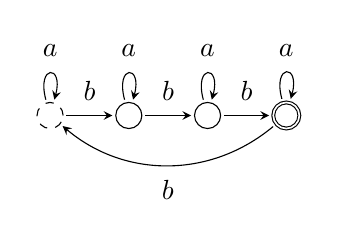
\begin{tikzpicture}
  [bend angle=40,every node/.style={draw,circle}]

  \tikzstyle{initial} = [dashed]

  \node[initial]   (1) at (1,0) {};
  \node            (2) at (2,0) {};
  \node            (3) at (3,0) {};
  \node[accepting] (4) at (4,0) {};

  \path[->, >=stealth, shorten > = 1pt, shorten < = 1pt]
        (1) edge              node[auto,draw=none] {$b$} (2)
        (2) edge              node[auto,draw=none] {$b$} (3)
        (3) edge              node[auto,draw=none] {$b$} (4)
        (1) edge [loop above] node[auto,draw=none] {$a$} (1)
        (2) edge [loop above] node[auto,draw=none] {$a$} (2)
        (3) edge [loop above] node[auto,draw=none] {$a$} (3)
        (4) edge [loop above] node[auto,draw=none] {$a$} (4)
        (4) edge [bend left]  node[auto,draw=none] {$b$} (1);
\end{tikzpicture}
\caption{The target} \label{fig:target}
\end{subfigure}
\hfill
\begin{subfigure}[b]{0.4\textwidth}
\centering
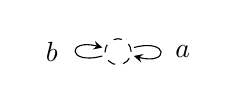
\begin{tikzpicture}
  [bend angle=40,every node/.style={draw,circle}]

  \tikzstyle{initial} = [dashed]

  \node[initial]   (1) at (1,0) {};

  \path[->, >=stealth, shorten > = 1pt, shorten < = 1pt]
        (1) edge [loop right] node[auto,draw=none] {$a$} (2)
        (1) edge [loop left]  node[auto,draw=none] {$b$} (2);
\end{tikzpicture}
\caption{First hypothesis} \label{fig:hypoth_1}
\end{subfigure}
\caption{Automata}
\end{figure}


\begin{table}
\centering

\begin{subtable}[h]{.23\textwidth}
\centering
\begin{tabular}{ | l || c | }
\hline
           & $\epsilon$ \\ \hline \hline
$\epsilon$ & $0$        \\ \hline \hline
$a$        & $0$        \\
$b$        & $0$        \\
\hline
\end{tabular}
\caption{} \label{tbl:observation_1}
\end{subtable}
%
%
\hfill
\begin{subtable}[h]{.23\textwidth}
\centering
\begin{tabular}{ | l || c | }
\hline
           & $\epsilon$ \\ \hline \hline
$\epsilon$ & $0$        \\
$b$        & $0$        \\
$bb$       & $0$        \\
$bbb$      & $1$        \\ \hline \hline
$a$        & $0$        \\
$ba$       & $0$        \\
$bba$      & $0$        \\
$bbba$     & $1$        \\
$bbbb$     & $0$        \\
\hline
\end{tabular}
\caption{} \label{tbl:observation_2}
\end{subtable}
%
%
\hfill
\begin{subtable}[h]{.23\textwidth}
\centering
\begin{tabular}{ | l || c | c | }
\hline
           & $\epsilon$ & $b$ \\ \hline \hline
$\epsilon$ & $0$        & $0$ \\
$b$        & $0$        & $0$ \\
$bb$       & $0$        & $1$ \\
$bbb$      & $1$        & $0$ \\ \hline \hline
$a$        & $0$        & $0$ \\
$ba$       & $0$        & $0$ \\
$bba$      & $0$        & $1$ \\
$bbba$     & $1$        & $0$ \\
$bbbb$     & $0$        & $0$ \\
\hline
\end{tabular}
\caption{} \label{tbl:observation_3}
\end{subtable}
%
%
\hfill
\begin{subtable}[h]{.23\textwidth}
\centering
\begin{tabular}{ | l || c | c | c | }
\hline
           & $\epsilon$ & $b$   & $bb$ \\ \hline \hline
$\epsilon$ & $0$        & $0$   & $0$  \\
$b$        & $0$        & $0$   & $1$  \\
$bb$       & $0$        & $1$   & $0$  \\
$bbb$      & $1$        & $0$   & $0$  \\ \hline \hline
$a$        & $0$        & $0$   & $0$  \\
$ba$       & $0$        & $0$   & $1$  \\
$bba$      & $0$        & $1$   & $0$  \\
$bbba$     & $1$        & $0$   & $0$  \\
$bbbb$     & $0$        & $0$   & $0$  \\
\hline
\end{tabular}
\caption{} \label{tbl:observation_4}
\end{subtable}
\caption{Observation tables}
\end{table}

Since the table is both closed and consistent, the algorithm moves on to phase two
and constructs the hypothesis of figure \ref{fig:hypoth_1}. It executes an
equivalence query with the hypothesis as parameter. Since it does not match $M$,
the oracle will provide a counterexample. Assume the counterexample provided is
$bbb$ (it could also have provided other counterexamples such as $bbbbbbb$).
Now, the counterexample and all prefixes are added to $S$. After performing the
new membership queries, the table \ref{tbl:observation_2} is built and the
algorithm returns to phase one.

The new table is closed, but not consistent, since $\row(b) = \row(bb)$, but
$\row(b \concat b)$ and $\row(bb \concat b)$ differ under the column $\epsilon$.
Therefore, $L^*$ adds $b \concat \epsilon = b$ to $E$, resulting in table
\ref{tbl:observation_3}. This table is still inconsistent, since $\row(\epsilon)
= \row(b)$, but $\row(\epsilon \concat b)$ differs from $\row(b \concat b)$ under
the column $b$. Therefore, $L^*$ adds $b \concat b$ to $E$. Performing the new
membership queries now results in table \ref{tbl:observation_4}. The table is
now both consistent and closed, so $L^*$ moves on to phase two and constructs the
hypothesis of figure \ref{fig:target}. Since this is equal to the target, the
equivalence query returns `yes' and the algorithm terminates.

\subsubsection{Complexity Analysis}
\label{sec:complexity-analysis-lstar}
% Note: Angluin considers k to be constant and therefore drops the term in the
% asymptotic upperbounds of both the query complexity and space complexity. She
% also does not explicitly state the required number of membership queries, but
% it is easy to see that this will be equal to the number of cells in the
% observation table.

Since the runtime complexity is dependent on the implementation of the queries
(which are application specific), it is more useful to consider the number of
queries made. Specifically, the number of membership queries, as these normally
far outnumber the equivalence queries. The asymptotic number of membership
queries is called the \textit{query complexity}.

Angluin states that the number of items in the observation table is at most
\begin{equation} \label{eq:obs_table_items}
(k+1)(n+m(n-1))n = \mathcal{O}(mn^2)
\end{equation}
In this equation $k = |\Sigma|$, $n$ is the number of states in the minimum
acceptor of the target and $m$ is equal to length of the longest
counterexample\cite{Angluin1987}. Since each item has a length of at most
$\mathcal{O}(m+n)$, she concludes that the total space required for storing the
observation table is $\mathcal{O}(m^2n^2 + mn^3)$.

In \cref{sec:improvements} various improvements are discussed. The complexities
of these improvements usually contain a term $k$. In order to be able to
directly compare these improvements to $L^*$, we need to slightly modify
Angluin's result. By keeping $k$ as a variable instead of a constant, the
upperbound of the number of items in the observation table is
$\mathcal{O}(kmn^2)$ (this follows directly from the left-hand side of equation
\ref{eq:obs_table_items}). We conclude that the query complexity is also
$\mathcal{O}(kmn^2)$, since for each item in the observation table exactly one
membership query is performed.\footnote{Angluin notes that the maximum number of
equivalence queries is $n$, thus for $L^*$ the membership queries indeed far
outnumber the equivalence queries.} The total space required for the observation
table becomes $\mathcal{O}(kmn^2) \cdot \mathcal{O}(m+n) = O(km^2n^2 + kmn^3)$.
This is equal to the total space complexity, since adding the space required for
the hypothesis (which is $\mathcal{O}(kn)$) does not change the complexity.

\end{document}

%%% Local Variables:
%%% mode: latex
%%% TeX-master: "main"
%%% End:
